 \begin{tikzpicture}[
          scale=1.0,>=stealth,domain=0.5:8,samples=100,
          declare function={
          xshift = 0.7;
          yshift = 0.3;
          gamma(\x) = 1.5/(\x+xshift)^2  +yshift;
          noise(\x) = 1.5*exp(-1.0*(\x+xshift))*cos(10*(\x+xshift) r);
          calcgamma(\x) = gamma(\x) + noise(\x);
        }]
     \small
%  \draw[very thin,color=gray] (-0.1,-0.1) grid (4.9,4.9);
  \draw[->,thick] (-0.2,0) -- (5.2,0) node[right] {$E$};
  \draw[->,thick] (0,-0.2) -- (0,4.2) node[above] {$\Gamma(E)$};
  % add ticks
  \draw [thick] (4,0) -- (4,-2pt) node [anchor=north] {$E_r$};
  \draw [color=black,domain=0:5,smooth,very thick]    plot
         (\x,{gamma(\x)}) node [anchor=south east] {density function};
  \foreach \x in {0.2,0.8,...,5}
    \fill[color=orange!80] (\x,{gamma(\x)}) circle (0.08);
  \foreach \x in {0.4,1.0,...,5}
    \fill[color=diplom1!80] (\x,{gamma(\x)}) circle (0.08);
  \foreach \x in {0.6,1.2,...,5}
    \fill[color=diplom2!80] (\x,{gamma(\x)}) circle (0.08);
%  \draw [color=red,domain=0.0:5,smooth,thick]    plot
%         (\x,{calcgamma(\x)}) node [above left=20pt] {real life};
 \end{tikzpicture}
 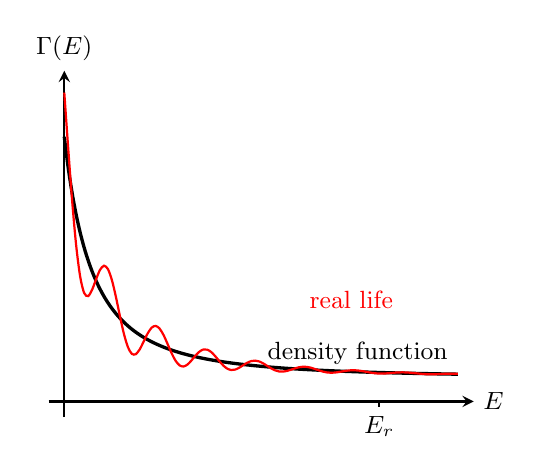
\begin{tikzpicture}[
          scale=1.0,>=stealth,domain=0.5:8,samples=100,
          declare function={
          xshift = 0.7;
          yshift = 0.3;
          gamma(\x) = 1.5/(\x+xshift)^2  +yshift;
          noise(\x) = 1.5*exp(-1.0*(\x+xshift))*cos(10*(\x+xshift) r);
          calcgamma(\x) = gamma(\x) + noise(\x);
        }]
     \small
%  \draw[very thin,color=gray] (-0.1,-0.1) grid (4.9,4.9);
  \draw[->,thick] (-0.2,0) -- (5.2,0) node[right] {$E$};
  \draw[->,thick] (0,-0.2) -- (0,4.2) node[above] {$\Gamma(E)$};
  % add ticks
  \draw [thick] (4,0) -- (4,-2pt) node [anchor=north] {$E_r$};
  \draw [color=black,domain=0:5,smooth,very thick]    plot
         (\x,{gamma(\x)}) node [anchor=south east] {density function};
%  \foreach \x in {0.2,0.8,...,5}
%    \fill[color=orange!80] (\x,{gamma(\x)}) circle (0.08);
%  \foreach \x in {0.4,1.0,...,5}
%    \fill[color=diplom1!80] (\x,{gamma(\x)}) circle (0.08);
%  \foreach \x in {0.6,1.2,...,5}
%    \fill[color=diplom2!80] (\x,{gamma(\x)}) circle (0.08);
  \draw [color=red,domain=0.0:5,smooth,thick]    plot
         (\x,{calcgamma(\x)}) node [above left=20pt] {real life};
 \end{tikzpicture}
